




\section{Presenting Task-Relevant Text}
\label{cp7:info-viz}




In Chapter~\ref{ch:assisting}, we described how \acs{tool}
highlights the text in a natural language artifact that it identifies 
as relevant to an input task. Our idea to highlight text 
draws from related work which suggests that textual highlights 
are a simple approach to surface the most important information in 
an artifact~\cite{Robillard2015,nadi2020}. 
Although simple, participants shared limitations of 
this strategy:



\smallskip
\begin{quote}
``\textit{It was much easier to follow with previously highlighted text.  
    However, it would have been nicer to have some sort of side bar/index of highlighted snippets
    where I could know and scroll directly through the highlighted parts of a page.}''
\end{quote}



\smallskip
\begin{quote}
``\textit{There was a resource page which was super long, and I found it very difficult to locate which sentences were highlighted, therefore, making that resource useless to me because I didn't have the motivation to scroll through it to find all highlights. An interface that gathers highlight locations would make a difference.}''
\end{quote}


\smallskip
This feedback made us question other potential ways to present the text identified by \acs{tool}.
For example, we could have followed design principles adopted by Unakite~\cite{Liu2018Unakite}---a tool that collects, organizes and keeps track of information---to make \acs{tool} display the text identified on its context menu.
Figure~\ref{fig:navigational-cues} shows a mock up of \acs{tool} bundling the highlights identified for one of the artifacts in the \texttt{titanic} task (Section~\ref{cp6:tasks}).
Using this context menu, a user could click on the text identified and navigate to the part of the documentation 
originally containing the text.



\begin{figure}
    \centering
    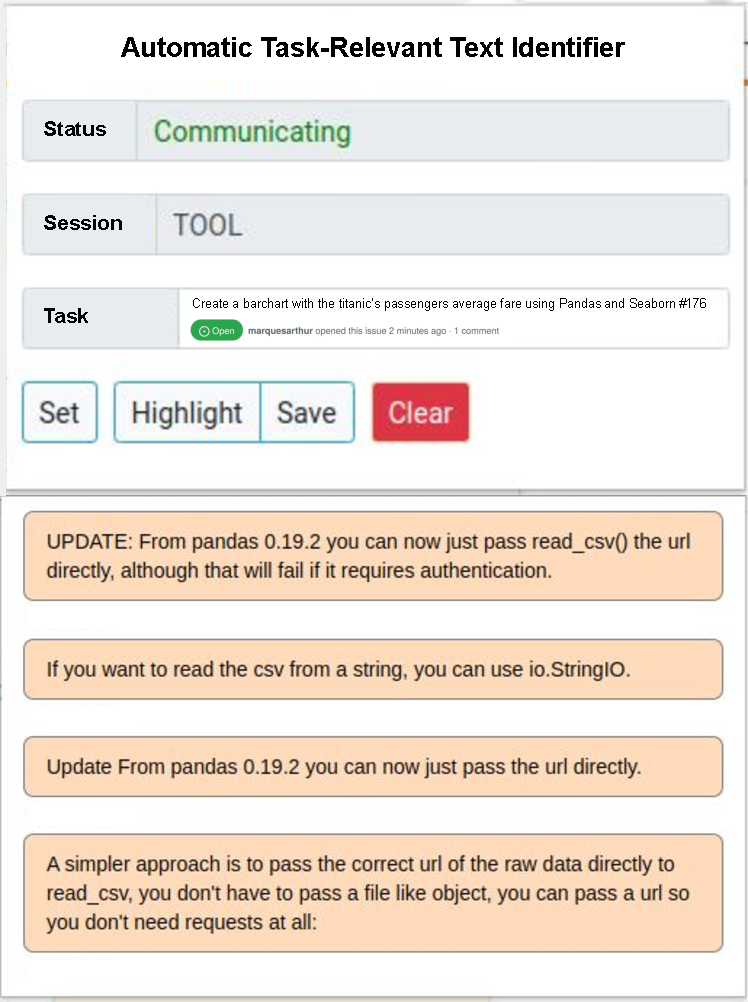
\includegraphics[width=0.45\textwidth]{fig/cp7/navigational-cues}
    \caption{Mock up of the highlights identified by \acs{tool} as navigational cues; by clicking on a highlight, a user could be directed to the part of a document containing that highlight}
    \label{fig:navigational-cues}
\end{figure}



A second approach to organizing the text identified could consider 
the semantic meaning of each sentence, as extracted through frame semantics or other semantic-based approaches. 
Semantic frames could 
assist a user in comprehending the content of the text automatically identified
without the need to read it. 
As done by Libra~\cite{Ponzanelli2017}, semantic frames could also be used to group the text identified in bubbles or a hierarchical representation 
 helping a developer
in deciding what portions of the text they would inspect first. 
Figure~\ref{fig:semantic-cues} shows a mock up 
with some of the semantic frames extracted 
for the sentences in Figure~\ref{fig:navigational-cues}.
Using the semantic frames identified,
a developer could decide whether they would read sentences 
describing some coding procedure (\textit{execution}), or sentences 
with warnings or requirements (\textit{requirement} and \textit{being obligated})
about the Pandas API. 
To be useful, future research must consider how to identify from all the frames available in a sentence, 
which frames
better summarize the meaning of the text. 


We leave the investigation of other ways to present the text identified as relevant to future research.




\begin{figure}
    \centering
    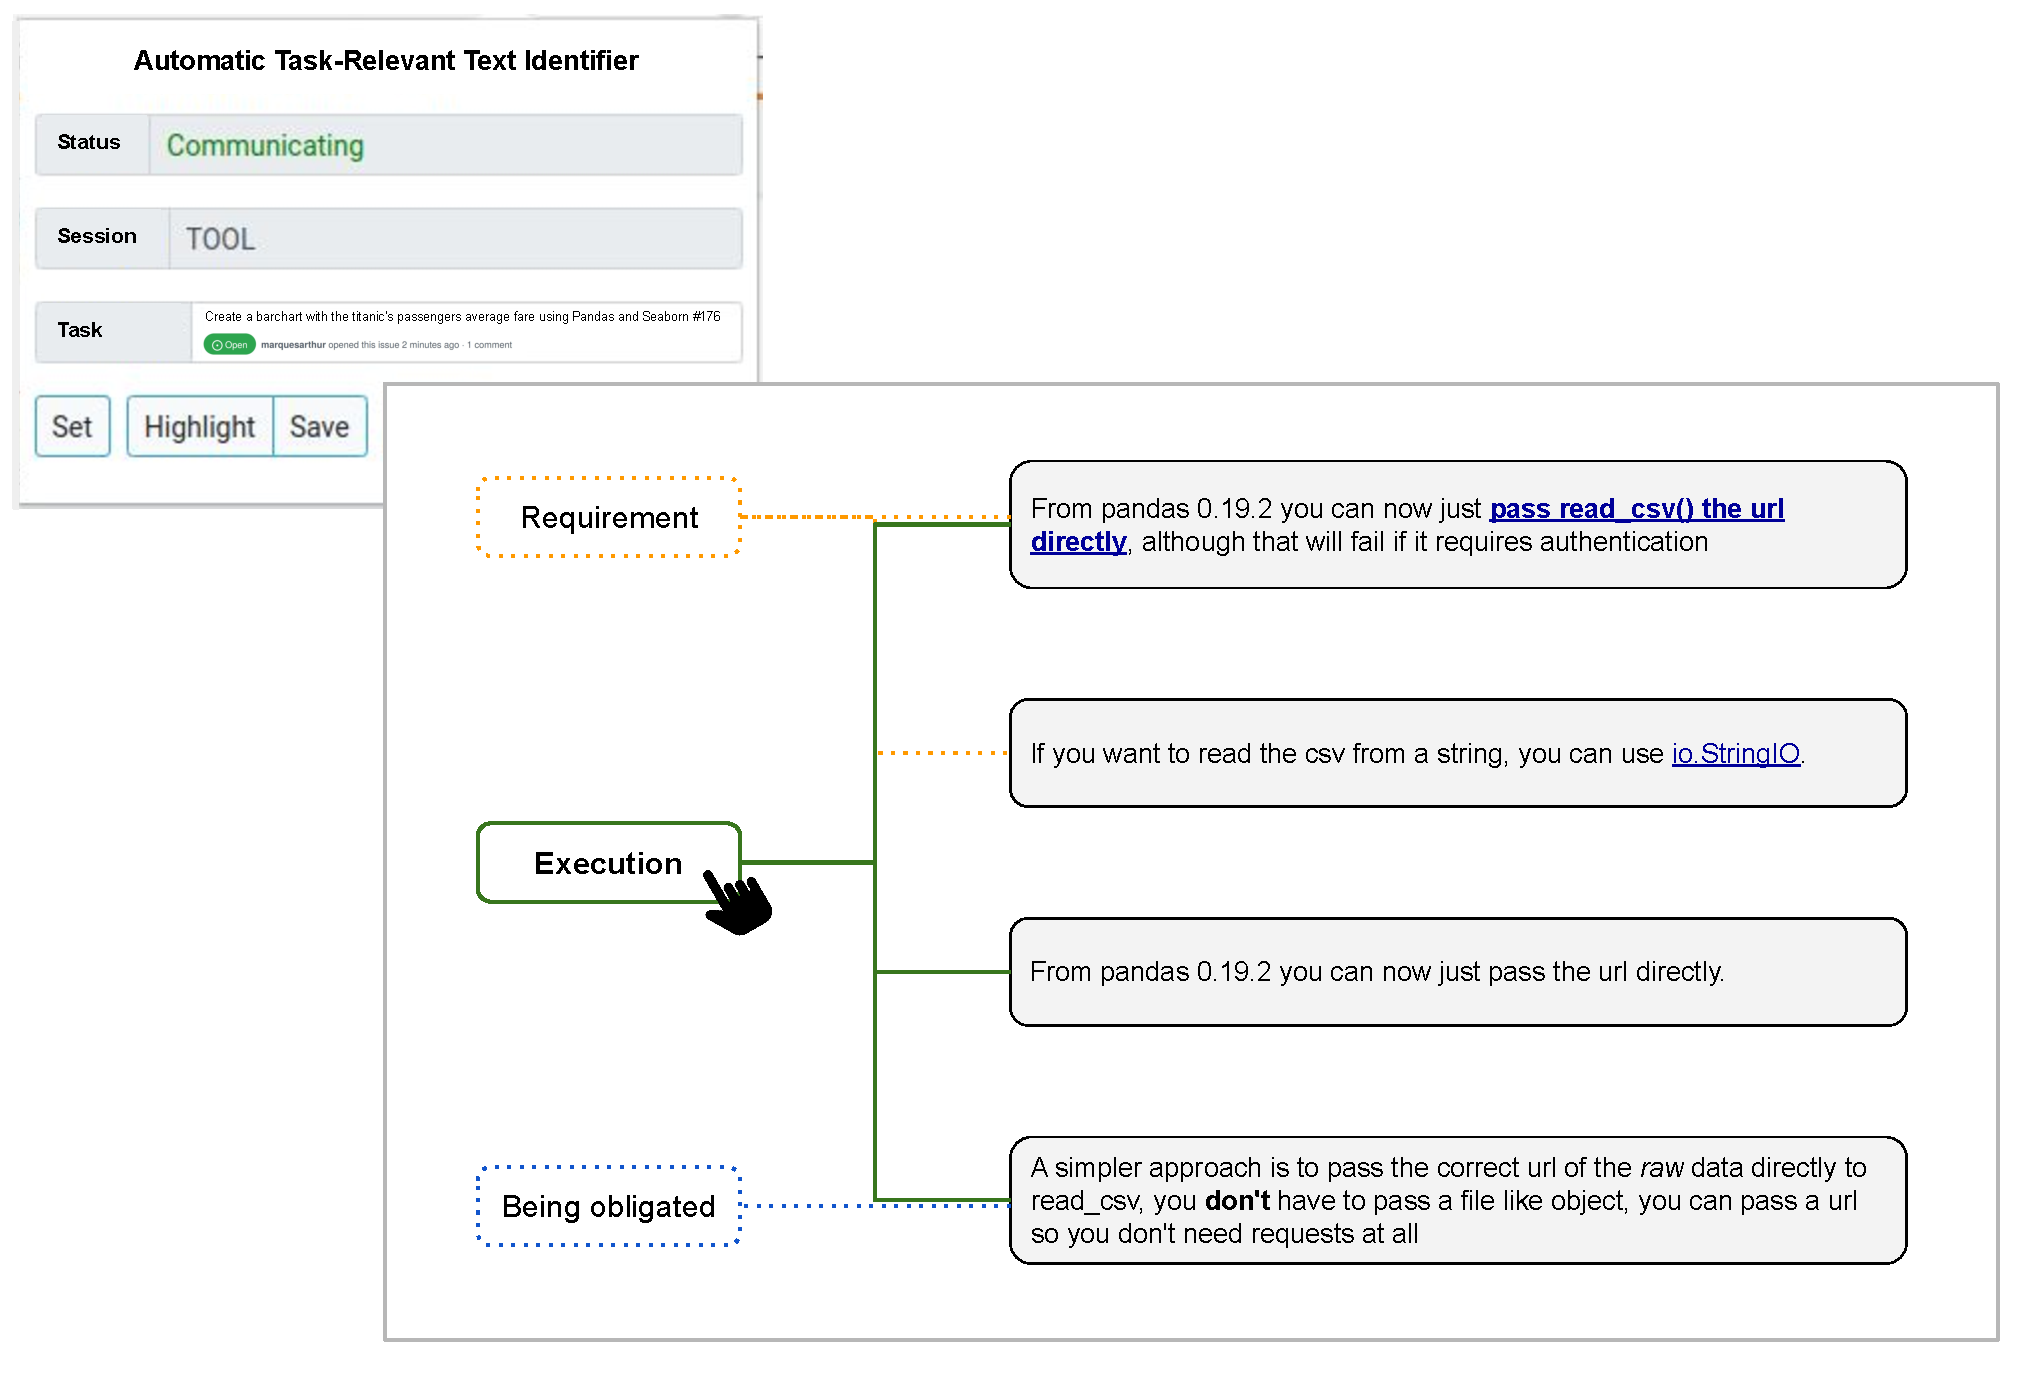
\includegraphics[width=0.90\textwidth]{fig/cp7/semantic-cues}
    \caption{Mock up of the highlights grouped by semantic frames; by hovering over a semantic frame, a user could quickly identify which of the text identified is associated with a certain meaning}
    \label{fig:semantic-cues}
\end{figure}





